\documentclass[english, a4, 12pt]{scrartcl}
%% encodings                                        
\usepackage[T1]{fontenc}                            
\usepackage[utf8]{inputenc}                         
\usepackage[shorthands=off]{babel}                  
\usepackage{lmodern}                                
\usepackage{microtype}                              
\usepackage{scrlayer-scrpage}                       
\usepackage{enumerate}                              
%\usepackage{enumitem}
\usepackage{csquotes}                               
\usepackage[backend=biber,style=numeric-comp]{biblatex}
\bibliography{bib.bib}

% %maths                                            
\usepackage{amsmath, amsthm, amssymb, bm, bbm, mathtools, dsfont, mathrsfs}

%commutative diagramms
\usepackage{tikz-cd}

% links, TODO
\usepackage[pdftitle={Seminar: "K1 von Ringen"},pdfauthor={Julian Seipel}, pdfsubject={Seminararbeit}]{hyperref}
%TODO: abschluss-projekt von tex-kurs heranziehen

                                                    
%special mathsymbols                                
\newcommand{\C}{\mathds{C}}                         
\newcommand{\R}{\mathds{R}}                         
\newcommand{\N}{\mathds{N}}                         
\newcommand{\Z}{\mathds{Z}}                         
\newcommand{\Q}{\mathds{Q}}
\newcommand{\pma}[1]{\begin{pmatrix} #1 \end{pmatrix}}
\newcommand{\A}{\mathscr{A}}
\newcommand{\F}{\mathbb{F}}                                                        
%\newcommand{\SS}{\mathbb{S}}
                    
%%%%%%%%%%%%%%%%%%%%                                
%theoremstyle                                       
%\theoremstyle{definition}                           
%\newtheorem*{Def}{Defintion}                        
%\theoremstyle{plain}                               
%\newtheorem{Beh}{Beh}                              
%\newtheorem{Vor}{Vor}                                                    
                          
% math (theorems)                     
\theoremstyle{definition}             
\newtheorem{Def}{Definition}[section] 
\newtheorem{Bsp}[Def]{Beispiel}       

\theoremstyle{remark}               
\newtheorem{Bem}[Def]{Bemerkung}      
\newtheorem{Wdh}[Def]{Wiederholung}   

\theoremstyle{plain}                  
\newtheorem{Satz}[Def]{Satz}          
\newtheorem*{satz}{Satz}              
\newtheorem*{Beh}{Behauptung}
\newtheorem{Lem}[Def]{Lemma}          
\newtheorem{Kor}[Def]{Korollar}       
\newtheorem{Fol}[Def]{Folgerung}      

%stuff used only a few times                        
\DeclareMathOperator{\f}{\varphi} 
\DeclareMathOperator{\GL}{GL}
\DeclareMathOperator{\SL}{SL}
\DeclareMathOperator{\K}{K_1}
\DeclareMathOperator{\SK}{SK_1}
\DeclareMathOperator{\E}{E}
\DeclareMathOperator{\Mat}{Mat}
\DeclareMathOperator{\diag}{diag}
% \newcommand{\exxp}[1]{\exp \left( #1 \right)}       
% \renewcommand{\sin}[1]{\sin \left( #1 \right)}      


%%% Local Variables:
%%% mode: latex
%%% TeX-master: "main"
%%% End:


%hilfmittelende

\begin{document}
\numberwithin{equation}{section}

	\begin{titlepage}
		\begin{minipage}[c][\textheight][c]{\textwidth}
			\begin{center}
				{ \Huge \textbf{Bachelorthesis} }
				
				\vspace*{1cm}
				{\Large Tamara Szecsey}
				
				\vspace*{1cm}
				{\Large \today}
				
				\vspace*{4cm}
				\hspace*{1cm} 
\includegraphics[height=30ex]{LOGO_UR}
			\end{center}
		\end{minipage}
	\end{titlepage}
	
\thispagestyle{empty}
\tableofcontents	
\clearpage	
\setcounter{page}{1}
\section{Introduction}
	\subsection{Conventions}
\section{Basic environments}
	
	%\subsection{Minkowski space}
	\subsection{Minkowski space \checkmark}
	First we need to know what a metric is. 
	The mathematical definition is as follows[see differentialgeometrie.pdf p.85]
	A metric
	$ d:X\times X \rightarrow \R$ is a function, that satisfies the conditions:
		\begin{enumerate}[(i)]
			\item $d(x,y)=d(y,x)$;
			\item $d(x,y)\geq 0$, with equality if and only if $x=y$;
			\item $d(x,y)+d(x,z)\geq d(x,z)$
		\end{enumerate}
	for any $x,y,z \in X$.
	 
	But in physics, we express the metric as an invariant line element:
		\begin{equation}
		 	\diff s^2 = g_{\mu\nu} \diff x^\mu \diff x^\nu
		\end{equation}
	so for getting $d(x,y)$ one have to take the square root of $\diff s^2$ and integrate. $g_{\mu\nu}(x)$ is the \textit{metric tensor}.
	 
	 For the of ordinary Minkowski space the metric tensor is now $g_{\mu\nu}(x) = \eta_{\mu\nu}$ so that
		\begin{equation}
			\diff s^2=- \diff t^2 + \diff x^2 + \diff y^2 + \diff z^2 = \eta_{\mu\nu} \diff x^\mu \diff x^\nu
		\end{equation}
	Where $\eta_{\mu\nu}$ is of the form

		\begin{equation}
		    \left(\eta_{\mu\nu}\right)=
		    \left(\begin{array}{cccc}
		    	-1 & 0 & 0 & 0\\
		    	0 & +1 & 0 & 0\\
		    	0 & 0 & +1 & 0\\
		    	0 & 0 & 0 & +1
			\end{array}\right)
%	    \begin{pmatrix}
%	    	-1 & 0 & 0 & 0\\
%	    	0 & 1 & 0 & 0\\
%	    	0 & 0 & 1 & 0\\
%	    	0 & 0 & 0 & 1
%	    \end{pmatrix}
		\end{equation}
	 
%%% Local Variables: 
%%% TeX-master: "main.tex" 
%%% End: 
 

	%\subsection{de Sitter space}
	\subsection{De Sitter space \checkmark} 
	De Sitter space is a good approximation of the geometry of our universe today and in the past while inflation\footnote{inflation: a well proofed theory of exponential expansion of space and mass in the early universe}. It is a solution of the Einstein's equations with positive energy and is a submanifold of the Minkowski space.
	
%	For defining a four-dimensional de Sitter space, we have a $(3+1)$-dimensional Minkowski space, where it would be a hyperboloid with \marginpar{siehe \cite{stringtheory_revolution} S.133}
%		\begin{equation}
%			\sum_{i=1}^4 (x^i)^2 - (x^0)^2 = R^2.			
%		\end{equation}
	
	In order to understand the form of the deSitter metric, let's start with the Riemann tensor\footnote{It should be known, that in general relativity we are in a four-dimensional Riemann manifold, where the Riemann tensor gives us the curvature.} for a \todo{was meint maximally symmetric} maximally symmetric n-dimensional manifold: 
		\begin{align}
			R_{\mu \nu \lambda \xi} = \kappa (g_{\mu \lambda} g_{\nu \xi} - g_{\mu \xi} g_{\nu \lambda})
		\end{align}
	Here $\kappa$ is a measure of the curvature.\footnote{It is normalized and more specifically, it's the Ricci curvature\todo{das ist falsch!! die ricci-krümmung ist gegeben durch R_ijki, mit summenkonvention, kappa ist hier wirklich für diesen speziellen fall einer riem. mannigfaltigkeit der wert der krümmung, du setzt mit maximal symmetrisch vorraus das die krümmung diese form hat.}, but this and more information about $\kappa$ is not needed for understanding the De Sitter space.}
	
	The already known Minkowski space is a maximally symmetric spacetime with a vanishing curvature $\kappa = 0$. If the curvature is positive, which means $\kappa > 0$, then it is called De Sitter space. For building its metric, we first take the five-dimensional Minkowski space:
		\begin{align}
			\d s^2_5 = -\d u^2 + \d x^2 + \d y^2 + \d z^2 + \d w^2
		\end{align}
	And a corresponding hyperboloid:
		\begin{align}
			-u^2 + x^2 + y^2 + z^2 + w^2 = 1
		\end{align}
	We use new coordinates $\tau, \chi, \theta$ and $\phi$:
		\begin{align}
			\begin{split}
			u &= \sinh (\tau) \\
			w &= \cosh (\tau) \cos \chi \\
			x &= \cosh (\tau) \sin \chi \cos \theta \\
			y &= \cosh (\tau) \sin \chi \sin \theta \cos \phi \\
			z &= \cosh (\tau) \sin \chi \sin \theta \sin \phi
			\end{split}
		\end{align}
	So in the end the metric on the hyperboloid looks like:
		\begin{align} \label{de-sitter}
			ds^2 = -\d \tau^2 + \cosh^2(\tau) \, \d \Omega^2_3 
		\end{align}
	with $\d \Omega_3^2 = \d \chi^2 + \sin^2 \chi (\d \theta^2 + \sin^2 \theta \d \phi^2)$
	which is the metric on a three-sphere $\Sp^3$.\footnote{A $n$-sphere is a $n$-dimensional manifold in Euclidean $(n+1)$~-~dimensional space. It´s the set of vectors with norm $1$}
	
	Just for completion, a maximally symmetric spacetime with negative curvature $\kappa < 0$ is called Anti-De Sitter space (further reading: \cite{SpacetimeCarroll}).
	 	
	%\subsection{Schwarzschild geometry}
	\subsection{Schwarzschild geometry \checkmark}
	
	The Schwarzschild geometry is a source-free solution of Einstein's equation \marginpar{[see chapter21 in ART Fließbach]} with spherical symmetry. The latter means, the solution is invariant under rotations. 
	At large distances it approaches the ordinary Minkowski space.
	The spacetime metric of the Schwarzschild geometry looks like this:\\
		\begin{equation} \label{p.3 (2.1)}
		\diff s^2=-\frac{r-2GM}{r}~ \diff t^2+\frac{r}{r-2GM}~
		\diff r^2+r^2 \left( \diff \theta^2+\sin^2\theta \diff \phi^2 \right).
		\end{equation}
	The G is Newton's gravitational constant, M is a mass parameter, which comes from idealisation if one is looking at the black hole from a distance $r\gg 2GM$.
	The term in the brackets is often shorten by $\diff \Omega_2^2$ which is on the two sphere $\Sp^2$.\footnote{A sphere is a n-dimensional manifold in Euclidean $(n+1)$~-~dimensional space.}
	
	The most interesting radii are $r=0$ and $r=2GM$.
	At $r=0$ we have a singularity, i.e. the sphere $\Sp^2$ goes to zero size and the Schwarzschild metric diverges.
	This can be described by the Riemann tensor $R_{\alpha\beta\gamma \delta}R^{\alpha\beta\gamma\delta}$ which encodes the tidal effects\footnote{tidal effects: The nearer an object is to a black hole, the more deformed it becomes because of the gravitational force. In the end, it will be destroyed before it reaches the singularity, except in Planck-scale physics.} on free-falling objects.
	
	$r_{s}\equiv 2GM$ is called the \textit{Schwarzschild radius}. At this radius, the metric has a singularity too, but that is just because of our choice of coordinates. Here the signs of $\diff r^2$ and $\diff t^2$ switch, so the coordinate $r$ becomes timelike, and the coordinate $t$ becomes spacelike. That causes that everything under $r_{s}$ will inevitably fall into the singularity. 
	So nothing, even massless particles like light, cannot move forward in ordinary time. This means for an observer in $r>r_{s}$, everything in $r<r_{s}$ is invisible and inversely. 
	
	That is, why $r_{s}$ is often called the \textit{event horizon} or just \textit{horizon}.
	In addition, the closer someone is to $r_{s}$ while sending a signal, the lower will be its energy when it reaches $r\gg 2GM$. This phenomenon is called \textit{gravitational redshift}.

			
%\clearpage		
\section{Basic ways of visualising the black hole problems on paper}
	
	%subsection{The Kruskal extenstion}
	\subsection{The Kruskal extension \checkmark (still questions)}
		\begin{figure}[htbp]
			\begin{center}
				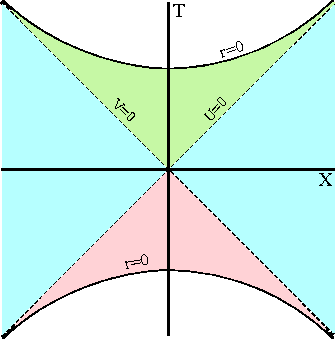
\includegraphics[scale=1]{kruskal}
			\end{center}
			\caption{This is the $XT$ plane of the \textbf{Kruskal extension}. The horizons are the dashed lines. The {\color{blue} blue} wedges are the exterior, the {\color{forestgreen} green} wedge is the future interior and the past interior is in {\color{red} red}. Nothing can escape the {\color{forestgreen} green} wedge into the {\color{blue} blue} wedges, because there is no radial null geodesic which would connect the wedges.}\label{kruskal}	
		\end{figure}
	From here on, we will use $r_{s}=2GM=1$.\footnote{This means, the Schwarzschild geometry looks like $\diff s^2=-\frac{r-1}{r} \diff t^2+\frac{r}{r-1}
		\diff r^2+r^2 \left( \diff \theta^2+\sin^2\theta \diff \phi^2 \right)$}
	Instead of using the coordinates $(t,r,\Omega)$ like in the previous section, we now introduce the Kruskal-Szekeres coordinates, because they are a better choice for near-horizon physics.
	
	First we parametrize the radial null geodesics in the Schwarzschild geometry as
		\begin{equation}
			t=\pm r_{*} + C,
		\end{equation}
	where C is some constant of motion and $r_{*}$ is a new radial coordinate defined as
		\begin{equation} \label{r_*tortoise}
			r_{*}\equiv r+\log (r-1).
		\end{equation}
	also called the \textit{tortoise coordinate}\footnote{The name \textit{"tortoise"} has its origin in the paradox of Achilles and the tortoise.}, because now we have an infinite coordinate range that fits in a finite geodesic distance.
		
	The Kruskal-Szekeres coordinates are then defined as
		\begin{equation}
			U\equiv -e^{\frac{r_*-t}{2}} \label{U}
		\end{equation}
		\begin{equation}
			V\equiv e^{\frac{r_*+t}{2}}.
		\end{equation}
	%\clearpage			%vllt mal Marei fragen, wie man das besser mit den footnotes machen kann
	Their lines of constant U and V are radial null geodesics and these coordinates have the property, that
		\begin{equation}
			 UV=(1-r)e^r.
		\end{equation}
	This means we have a singularity at $UV=1$ and the horizon is at $U=0$ or $V=0$. The metric looks now like
		\begin{equation}
			\diff s^2=-\frac{2}{r}e^{-r}\left(\diff U \diff V + \diff V \diff U\right)+r^2 \diff \Omega^2_{2}
		\end{equation}
	Because this metric still has an off-diagonal tensor, we define another set of coordinates
		\begin{equation}
		\begin{split}
			U=T-X 	\\	
			V=T+X
		\end{split}
		\end{equation}
	Now the metric looks as follows:
		\begin{equation}\label{SchXT}
			\diff s^2=\frac{4}{r}e^{-r}\left(- \diff T^2+ \diff X^2\right)+r^2 \diff \Omega^2_2
		\end{equation}
	Note that there is now no singularity at $r=1$.
	
	This metric defines a geometry over the full XT plane, which can be seen in Figure \ref{kruskal}. The \textbf{right {\color{blue} blue} wedge} is, in the old Schwarzschild coordinates, former $r>1,~-\infty<t<\infty$. If one wants to continue to $r<1$, there is a branch cut \marginpar{wie sieht dieser branch cut genau aus?} defined in \eqref{U}, which allows us to either go to the regions with $X^2-T^2<0$ and $T>0$ which is the \textbf{{\color{forestgreen} green} wedge}, or the \textbf{{\color{red} red} wedge} with $T<0$ and also $X^2-T^2<0$. At last we have the left {\color{blue} blue} wedge in which we also can have $r\gg1$. Both blue wedges are asymptotically Minkowski regions. 
	
	The singularity $r=0$, which you find at the top and the bottom of \textbf{Figure \ref{kruskal}}, is the hyperboloid $X^2-T^2=-1$. It has two connected components, one at each boundary of the {\color{forestgreen} green} and the {\color{red} red} regions. These two regions are also called the {\color{forestgreen} future} and the {\color{red} past} interiors, while the other two are called the original/new exteriors (right/left {\color{blue} blue} wedges).
	
	All regions together can interpret the full Schwarzschild metric as a wormhole connecting two nearly flat universes, both acting at $r\gg1$ as if there were a point source of mass $M$. Signals can not travel through the wormhole, but two observers coming from opposite sides could meet in the middle and compare notes. \marginpar{how the hell does he know that?}
	
	%subsection{Penrose diagrams} including supsupsections
	\subsection{Penrose diagrams}
%\FloatBarrier
	We want to know the causal structure of spacetime by asking the question which points can receive signals from which other points. 
For throwing out some irrelevant information, we will know introduce the so called \textit{conformal compactification}.
\begin{figure}[tbp]	
		\begin{center}
		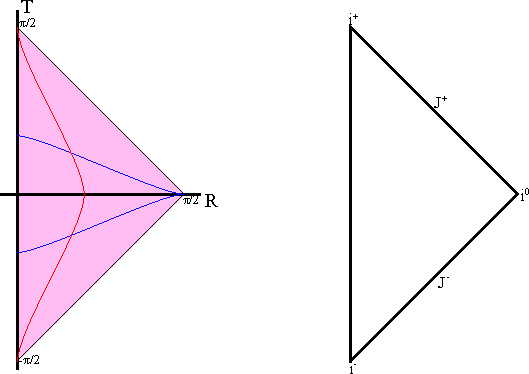
\includegraphics[scale=1]{flatpenrose}
		\end{center}
		\caption{On the left you see the full \textbf{Minkowski space} in pink in the RT plane. We removed the prefactor of \eqref{TRmetric}, because it would diverge at the boundary. On the right we formalize this in to a \textbf{Penrose diagram}.}\label{flatpenrose}
		\end{figure}
%hiermit bin ich noch nicht zufrieden!!!
\parbox{\linewidth}{~}
\hfill
\parbox{0.02\linewidth}{~}
\begin{minipage}[][][c]{0.96\textwidth}
We have two spacetimes with metrics, which are related as $g'_{\mu\nu}(x)=e^{2\omega(x)}g_{\mu\nu}(x)$ with a smooth real function $\omega(x)$. Or in other words, they differ only by multiplication with a positive scalar function on spacetime. The important thing is, those metrics have the same null geodesics.
This goes not without saying, because only timelike/spacelike curves in one metric will be timelike/spacelike curves in the other, but not geodesics.
Two metrics with this kind of relation are called \textit{conformally equivalent}. 
This gives us a way to represent the asymptotic behaviour of spacetimes at large distances.
\end{minipage}
\hfill

\parbox{\linewidth}{~}%hier Abstände nicht verändern!

Now, \textit{conformal compactification} is including infinity as a boundary of spacetime in a manifold by taking a function $\omega(x)$ that diverges while we approach infinity, so that infinity is brought into a finite distance.
\marginpar{sollten metriken damit nicht auch was zu tun haben?}

	\subsubsection{of Minkowski space \checkmark}
		%\clearpage		
		
	We will now show this on an example, the ordinary flat Minkowski space, whose metric in spherical coordinates looks like
		\begin{equation}
			\diff s^2=- \diff t^2+ \diff r^2+r^2 \diff \Omega^2_2
		\end{equation}
	Because the interesting things are happening in the asymptotical behavior at $r \rightarrow \infty$ and $|t| \rightarrow \infty$, we parametrize them with the aid of $\arctan(x)$, so that the boundary is pulled in a finite distance.
		\begin{equation}
		\begin{split}
			T+R\equiv\arctan(t+r) \\
			T-R\equiv\arctan(t-r)
		\end{split}
		\end{equation}
	
	And now the metrics looks as follows:
		\begin{equation} \label{TRmetric}
			\diff s^2=
			\frac{1}{\cos^2(T+R)\cos^2(T-R)}
			\left[- \diff T^2+ \diff R^2+\left(\frac{\sin(2R)}{2}\right)^2 \diff \Omega^2_2 \right].
		\end{equation}	
					
%		\begin{figure}[tbp]	
%		\begin{center}
%		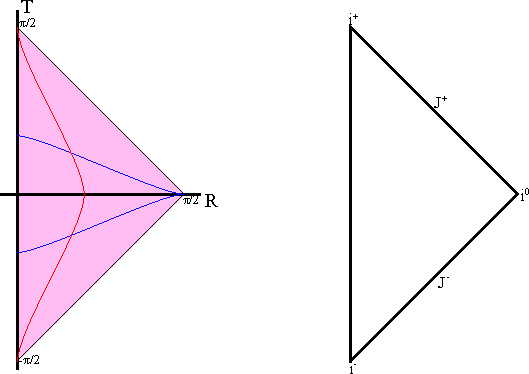
\includegraphics[scale=1]{flatpenrose}
%		\end{center}
%		\caption{On the left you see the full \textbf{Minkowski space} in pink in the RT plane. We removed the prefactor of \eqref{TRmetric}, because it would diverge at the boundary. On the right we formalize this in to a \textbf{Penrose diagram}.}\label{flatpenrose}
%		\end{figure}
	This seems to be quite complicated, but if you have a look at \textbf{Figure \ref{flatpenrose}}, you will see, why we were doing this. The new ranges of our coordinates are $|T \pm R|< \pi/2, R\geq0$, and the spacetime was compactified by including the boundary at $|T \pm R| = \pi/2$. 
	
	The new boundary which are illustrated in \textbf{Figure \ref{flatpenrose}} on the right side, is divided into five parts:	
		\begin{tabbing}
			\hspace{0.1\linewidth} \= \hspace{0.4\linewidth} \= \hspace{0.1\linewidth} \= \hfill \kill
			$i^+$~~: \> future timelike infintity\> $J^+$~~: \> future null infinity \\
			$i^-$~~: \> past timelike infinity \> $J^-$~~: \> past null infinity\\
			\hspace{0.35\linewidth} \= \hspace{0.1\linewidth} \= \hfill \kill	
			~ \> $i^0$~~: \> spatial infinity 
		\end{tabbing}
	So timelike curves come from $i^-$ and go to $i^+$, same for null curves with $J^\mp$, the spatial geodesics are ending at $i^0$. Massless particles are entering/leaving at $i^\mp$ and massive particles at $J^\mp$. The scattering matrix\footnote{also called S-matrix} maps the states on $J^- \cup i^-$ to the states on $J^+ \cup i^+$.	
	
	Out of the diagram, we can see, that the Minkowski space does \textit{not} have \textit{event horizons}.
	%\clearpage
	
	\subsubsection{of de Sitter space \textbf{N}}
	\begin{figure}[tbp]
	 	\begin{center}
			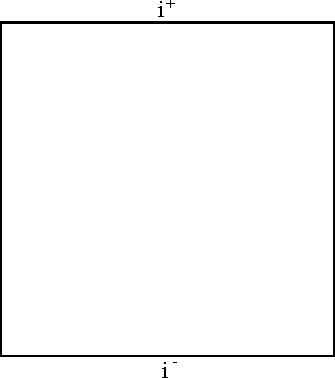
\includegraphics[scale=0.8]{dspenrose}
		\end{center}
	  		\caption{Beschreibung}\label{dspenrose}
	\end{figure}
	Its metric is:
		\begin{equation}
			\diff s^2=- \diff \tau^2+\cosh^2\tau \diff \Omega^2_3
		\end{equation}
		Now we know, that de Sitter space has no infinite spatial boundary $i^0$, nor any light-like infinity $J^\mp$. That means, it is too complicated to find a formulation of de Sitter space in quantum theory and finding a S-matrix may be impossible. 
		
		But it has \textit{event horizons}! That means, observers, who are moving on timelike geodesics at vertical straight lines in the diagram \textbf{Figure \ref{dspenrose}.} could be unable to communicate.
	 
	%\FloatBarrier
	\subsubsection{of Schwarzschild geometry \textbf{N}}
	
	For the Penrose diagram of the Schwarzschild geometry, we take the Kruskal Szekeres coordinates of \eqref{SchXT}. That lightens the compactification we need for the Penrose diagram a lot, because the difference between $(T,X,\Omega)$ coordinates and the Minkowski space coordinates $(t,r,\Omega)$ is just their range.\footnote{Minkowski: $-\infty < t < \infty, r\geq 0$; Kruskal: $X^2-T^2 > 1$}
	So the transformation is as it was for Minkowski space:
		\begin{equation}
			\begin{split}
			T'+X'\equiv \arctan(T+X) \\
			T'-X'\equiv \arctan(T-X)
			\end{split}		
		\end{equation}
	But instead we have now the coordinate range of $|X'\pm T'|< \pi/2$ and $|T|< \pi/4$ \marginpar{? warum $|T|$ und nicht $|T'|$}
	If you draw this into a diagramm, it looks like the Kruskal diagram in \textbf{Figure \ref{kruskal}}, but now the spacetime boundaries are shown too.
		\begin{figure}[tbp]  	
	  	\begin{center}
		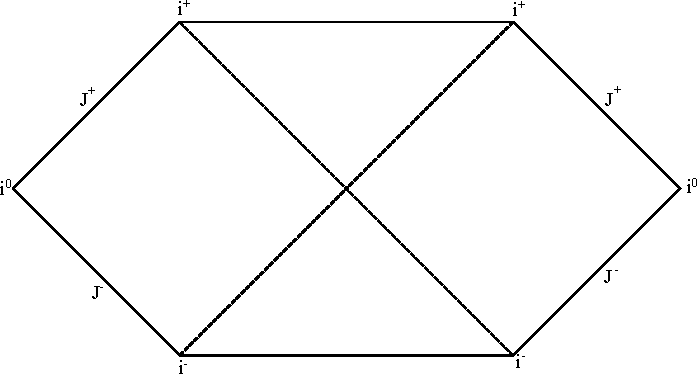
\includegraphics[scale=1]{schpenrose}
		\end{center}
		\caption{This is the \textbf{Penrose diagramm} for the \textbf{Schwarzschild geometry}. The horizons are marked in dashed lines. As you can see, there are boundaries like the ones of the Minkowski space on both sides.}
		\end{figure}
	\FloatBarrier

		

	%subsection{Classical black hole formation}	
	\subsection{The apparant horizon N}
	\begin{figure}[tbp] 
		\begin{center}
			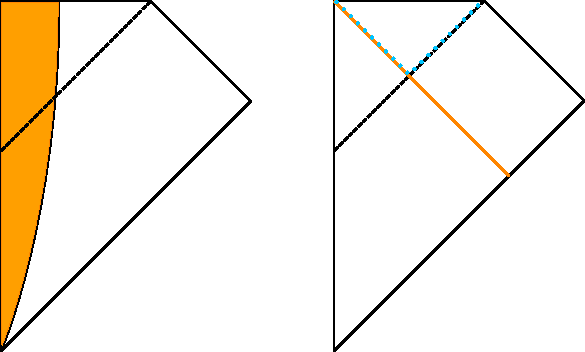
\includegraphics[scale=1]{collapse}
		\end{center}
			\caption{In both diagrams, the upper boundary is the singularity while the left boundary is the origin of the polar coordinates. The other two boundaries are asymptotic to the ones of the Minkowski space. On the left side we have a collapsing cloud of massive particles shown in orange, which forms the black hole. On the right side we have a black hole forming out of an infalling shell of photons, where we have the Schwarzschild geometry above the orange line, and a piece of Minkowski space below it. The event horizon is illustrated as a dashed line, the apparent horizon is shown with blue dots.}\label{collapse}
	\end{figure}	
	Now, how does that lead us to black holes? First of all, real astrophysical black holes are a result of gravitational collapse, like at the end of a star live. But considering massive particles would mean, that we have to include all interactions between them. So for making it convenient, we instead imagine a black hole arise from a spherically symmetric infalling shell of photons. 
	That also leads to the fact, that there is no obstacle while the black hole is formed, like the Schwarzschild radius.
		
	But now the horizon extends into the Minkowski space and we have to make a difference between the \textit{actual horizon} and the \textit{apparent horizon}.
	When you are passing the actual horizon, you will not notice it immediately, even though your fate has already been sealed. This leads to some kind of acausal nature of horizons: Their locations depend on events that have not yet happened. 
	
	For defining the apparent horizon, which will help us, to avoid this acasual nature, we first notice, that the Schwarzschild horizon can be detected locally in time, for any sphere of constant $r$ with $r<1$.\footnote{Here, the Schwarzschild radius is set to $2GM=1$}
	Any null geodesics of these spheres which starts out orthogonal, converges towards other null geodesics of this kind. And if we have a compact 2-dim surface, it is called a \textit{closed trapped surface}.
	
	\textbf{An apparent horizon is now a surface which is a boundary of a connected set of closed trapped surfaces.}
	For to describe the real black hole in one diagram, we take a mixture of Minkowski space and Schwarzschild solution into a Penrose diagram as shown in \textbf{Figure \ref{collapse}.} The apparent horizon is illustrated with blue dots. And as you can see, it does form itself in the same moment when the photon shell crosses the event horizon.
					

%\section{What is Quantum field theory?}
\section{What is Quantum field theory? \checkmark} \label{QFT}
	Here the Hilbert space is like an infinite tensor product over all points in space, while we have finite degrees of freedom at each point. 
For example, we take a scalar field $\phi(x)$ where there is only a one degree of freedom at each spatial point. 

	Then the free scalar field of mass m's Hamiltionian looks like
		\begin{equation}
			H=\frac{1}{2}\int \diff^3 x \left(\pi(x)^2 + \vec{\nabla}\phi(x) \cdot \vec{\nabla}\phi(x) + m^2\phi(x)^2 \right).
		\end{equation}
	The function $\pi(x)$ is the canonical conjugated momentum to $\phi$ which can be put out to tender as $\frac{\partial \mathscr{L}}{\partial \dot{\phi}(x)}$. For beginners, the $\phi$ would be something like the spacial coordinate $x$ in theoretical mechanics and $\pi$ is the companion piece to $p$, the momentum.
	Together they obey
		\begin{align}
			\begin{split}
				[\phi(x),\pi(y)]&=i \delta^3(x-y) \\
				[\phi(x),\phi(y)]&=0 \\
				[\pi(x),\pi(y)]&=0.
			\end{split}
		\end{align}
	This is consistent to the fact that for each field at a each point, we have an individual tensor factor. Note that x and y are four dimensional coordinates living in Minkowski space.
			
	The Hamiltonian results out of the Lorentz-invariant action\footnote{For germanspeakers: Because it is often confused because of television, action in physics means \textit{Wirkung}.}:
		\begin{equation}
			S=-\frac{1}{2} \int \diff^4 x \left(\partial_\mu \phi \partial^\mu \phi + m^2\phi^2 \right)
		\end{equation}
	Where in general action is defined as \cite{MechanikFliesbach}: 
		\begin{equation} 
			S=S[q]= \int\limits_{t_1}^{t_2} \diff t \mathscr{L}(q,\dot q,t)
		\end{equation} 
	In quantum mechanics, we are often interested in describing the ground state wavefunction $|\Omega\rangle$. If we do this for the free massive scalar field, we find that \marginpar{[7]}
		\begin{equation}
			\langle\phi| \Omega\rangle \propto \exp\left[-\frac{1}{2} \int \diff^3 x \diff^3 y \phi(x)\phi(y) K(x,y)\right].
		\end{equation}
	with
		\begin{equation}
			K(x,y)=\int \frac{\diff^3 k}{(2\pi)^3} e^{i\vec{k} \cdot (\vec{x}-\vec{y})} \sqrt{\vec{k}^2+m^2}.
		\end{equation}
	%Here $r \equiv |x-y|$.	
	$K(x,y)$ is a propagator and normally includes at least four coordinates, two for the beginning state and two for the final state. If we want to include time-ordering, we would use the Green's function which would be a Heaviside step function multiplied with this propagator: $G(\textbf{r}_2,t_2;\textbf{r}_1,t_1)=\Theta(t_2-t_1)\cdot K(\textbf{r}_2,t_2;\textbf{r}_1,t_1)$.\cite{QEDbuch}\\
	
	But we now would like to generalize theories with interactions, so we study the vacuum expectation values of products of Heisenberg picture fields which look like $\phi(t,x) \equiv e^{iHt} \phi(x) e^{-iHt}$. In our case of the free massive scalar field we have this solution of equation of motion:
		\begin{equation}  \label{EqOfMotion}
			\phi(t,\vec{x}) = \int \frac{\diff^3 k}{(2\pi)^2} \frac{1}{\sqrt{2\omega_k}} 
			\left[ a_{\vec{k}} e^{i(\vec{k}\cdot\vec{x}-\omega t)} +
			a^{\dagger}_{\vec{k}} e^{-i(\vec{k}\cdot\vec{x}-\omega t)}
			\right]
		\end{equation}
	where we defined $\omega_k \equiv \sqrt{\vec{k}^2+m^2}$. The $a^{\dagger}_{\vec{k}}$ and $a_{\vec{k}}$ should be known out of the basics of quantum mechanics as the creation and annihilation operators\footnote{They are defined: $\hat{a}= \sqrt{\frac{m\omega}{2\hbar}} 
		\left(\hat{q} + \frac{i}{m\omega}\hat{p}
		\right)
		$ and 
		$ \hat{a}^{\dagger}= \sqrt{\frac{m\omega}{2\hbar}} 
		\left(\hat{q} - \frac{i}{m\omega}\hat{p}
		\right)
		$
	with the feature that if you let them operate with a wave function $|n\rangle$ they act like this:
	$\hat{a}|n\rangle = \sqrt{n}|n-1\rangle$ and $\hat{a}^{\dagger}|n\rangle= \sqrt{n+1}|n+1\rangle$.
	And $a^{\dagger}$ is the adjoint of $a$ which means: $\langle \psi | a | \phi \rangle^*= \langle \phi | a^{\dagger} | \psi \rangle$ just for reminding.
%end footnote
	}, and they obey
		\begin{align*}
			[a_{\vec{k}},a^{\dagger}_{\vec{k'}}]&= (2\pi)^3 \delta^3 (\vec{k}-\vec{k'})\\
			[a_{\vec{k}},a_{\vec{k'}}]&=0 \\
			[a^{\dagger}_{\vec{k}},a^{\dagger}_{\vec{k'}}]&=0 \\
			[H,a_{\vec{k}}]&=-\omega_k a_{\vec{k}}.
		\end{align*}
	Now we are searching for a more abstract form of \eqref{EqOfMotion} where $a_n$ and $a^{\dagger}_n$ have the standard algebra, in the following way:
		\begin{equation} \label{wave_fct}
			\phi = \sum_n \left(f_n a_n + f^*_n a^{\dagger}_n \right)
		\end{equation}
	Here we use a basis of solutions $f_n(x)$ of
		\begin{equation} \label{Klein-Gordon-eq}
			\left( \partial_{\mu}\partial^{\mu} - m^2 \right) f(t,\vec{x})=0
		\end{equation}			
	that have a time dependence of the form $e^{-i\omega t}$ with $\omega>0$. We also define the same $f_n$ in a way, that they are orthonormal in the Klein-Gordon\footnote{Perhaps you already noticed, that \eqref{Klein-Gordon-eq} is the Klein-Gordon Equation which is nothing else than the relativistic Schrödinger Equation. It is just valid for spin 0 particles.} norm, so that
		\begin{equation} \label{KG-norm}
			(f_1,f_2)_{KG} \equiv
			i \int d^3x \left( f^*_1 \dot{f}_2 - \dot{f}^*_1 f_2
			\right).
		\end{equation}
	Now we can have a look at the expectation values (perhaps you remember, that this is the interesting part), which are called \textit{correlation functions}. With just a one-point function, it has to vanish
		\begin{equation}
			\langle \Omega| \phi(t,\vec{x}) |\Omega \rangle = 0.
		\end{equation}
	because of the translation invariance in vacuum and how $a_n$ and $a^{\dagger}_n$ act on the vacuum. In other words, it is forbidden, that one particle just arise from the vacuum but never vanishes oder that one particle had always existed end suddenly disappears. This is, why Quantum field theory is called a multiparticle theory.
	
	For a two-point function with equal times it looks like this:
		\begin{equation} \label{correlationfct}
			\langle \Omega| \phi(0,\vec{x})\phi(0,\vec{y}) |\Omega\rangle=
			\frac{1}{4\pi^2}\frac{m}{|\vec{x}-\vec{y}|}K_1(m|\vec{x}-\vec{y}|).
		\end{equation}
	This function scales with 
		\begin{itemize}
			\item[•] $\frac{1}{|\vec{x}-\vec{y}|}$ for $|\vec{x}-\vec{y}| \ll m^{-1}$
			\item[•] $e^{-m|\vec{x}-\vec{y}|}$ for $|\vec{x}-\vec{y}| \gg m^{-1}$
		\end{itemize}
	but is "gapless" for $m=0$, because the $m^{-1}$, which is also called \textit{correlation length}, is infinite, so exicted states' energies can be arbitrarily close to the ground state energy. A massless scalar field is also invariant under the \textit{conformal group}. This means here we can scale the spacetime like $x'^\mu = \lambda x^\mu$, so it's scale-invariant. The quantum field theory with this larger symmetry group is called \textit{conformal field theory} or \textit{CFT}.
	
	$K_1(m|\vec{x}-\vec{y}|)$ is some hyperbolic Besselfunction which is in general a solution of differential equation like the Klein-Gordon equation in hyperbolic coordinates. It contains an exponential function, which is, why we have the second point in the listing above. But I will not do further explanations about this function because it is not necessary here. \\
	
	We need to mention that \eqref{correlationfct} is a correlation function which is not only just valid in free scalar field theory but also is divergent in short distance power-law. 
	
	Now that we contemplate the two-point function without the time, we add the time difference to our calculations. But we need to order the function in time so we use the time-ordering operator $T$, so that the two-point function now is:
		\begin{equation}
			\langle \Omega| T \phi(t,\vec{x})\phi(t',\vec{y}) |\Omega\rangle=
			\frac{1}{4\pi^2} \frac{m}{\sqrt{|\vec{x}-\vec{y}|^2-(t-t')^2+i\epsilon}}
			K_1 \left( m\sqrt{|\vec{x}-\vec{y}|^2-(t-t')^2+i\epsilon}\right)
		\end{equation} 
	This is also called a \textit{transition amplitude}. T takes care that time increases while going left\marginpar{I think going left in a feynman diagram, but i am not sure}. The factor $\epsilon$ should go to zero and reminds us, that there could be other ways of complex integration because of the square root not leading to the timelike-seperated points.	

%\section{What is Entanglement and what is it good for?}
\section{What is Entanglement and what is it good for? \textbf{N}}
	 \begin{figure}[tbp]
	 	\begin{center}
	 		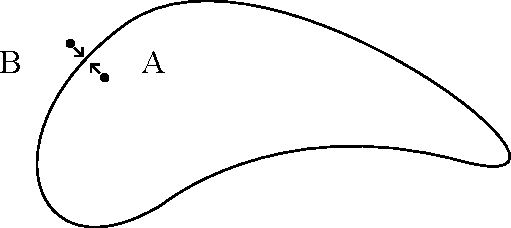
\includegraphics[scale=1]{entangledcorr}
	 		\caption{The boundary between these two regions is called the \textit{entangling surface}.}
	 	\end{center}
	 \end{figure}
	In relativistic QFT, the ground state has correlations between field operators at spatially separated points. Here we can use \textit{entanglement} as an explanation.
	
	But at first, let's start from the beginning:
	\\
	We have $\rho$ which is called \textit{density matrix} and is a quantum state on Hilbert space $\Hil$. Quantum states are illustrated in operators, here: $\rho$ is a non-negative hermitian one of trace 1. If it can be written in the form\footnote{Here $|\psi\rangle$ is some element of $\Hil$ with norm 1.}
		\begin{equation}
			\rho=|\psi\rangle \langle\psi|,
		\end{equation}
	 the quantum state is called \textit{pure}. If a state is not pure, it is \textit{mixed}.
	 
	 While doing an experiment, we will a measure a outcome $i$, which is always related to a projection operator $\Pi_i$ with a probalbility of measuring $i$, that looks like: 
		 \begin{equation}
	 		P(i)=\mathrm{tr}(\rho\Pi_i).
	 	\end{equation}
	 
	 For to find out, whether a given state $\rho$ is pure or mixed, we define a function $S$ for convenience:
		\begin{equation}
			S(\rho)\equiv -\mathrm{tr}(\rho \log \rho)
		\end{equation}	 	
	And $S(\rho)$ is called the \textit{Von Neumann Entropy} or \textit{information entropy}. 
	Its proberties are:
	\begin{itemize}
		\item[•] for any unitary operator $U$: $S(U^\dagger \rho U)=S(\rho)$
		\item[•] $S(\rho)\geq 0$, with equality if and only if $\rho$ is pure. 
		\item[•] for $d$ is the dimension of $\Hil$: $S(\rho)\leq \log d$, with equality if and only if $\rho$ is maximally mixed.
		\item[•] The entropy of the average over a set of states is at least equal to the average of all their individual entropies. This is also called \textit{concavity} and is definde as:
		\begin{equation}
			S \left(\sum_i \lambda_i \rho_i \right) \geq \sum_i \lambda_i S(\rho_i),
		\end{equation}
	while $\lambda_i$ is any set of non-negative numbers with $\sum_i \lambda_i =1$.
	\end{itemize}
	Now, let's have a look at an entangled state written in the two-qubit state:
		\begin{equation}
			|\Psi\rangle = \frac{1}{\sqrt{2}} \left(|00\rangle + |11\rangle \right)
		\end{equation}
	Here, the full state is pure, but the reduced state on either qubit ($|00\rangle$ or $|11\rangle$) is mixed. 
%	Bipartite systems are the ones whose Hilbert space can be written as a tensor product\footnote{Watch out! The tensor product $\otimes$ is not the direct sum $\oplus$.}:
%	 	\begin{equation}
%	 		\Hil=\Hil_A \otimes \Hil_B
%	 	\end{equation}
%	 In quantum mechanics they describe the composition of two independent physical systems and can be \textit{entangled}, which means, that the reduced density matrices $\rho_A$ and $\rho_B$ can be mixed even if the joint state $\rho_{AB}$ is pure.
%	 

\FloatBarrier 

%\section{Rindler}
\section{Rindler decomposition}
\FloatBarrier
		\begin{figure}[tbp]
			\begin{center}
				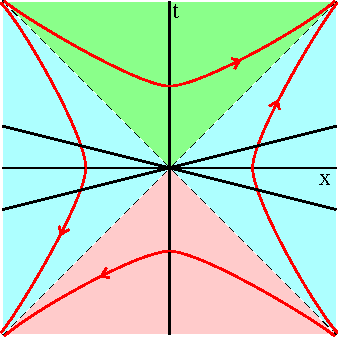
\includegraphics[scale=1]{boost}
				\caption{The \textbf{Rindler decomposition} of \textbf{Minkowski space}. The blue wedges are the Rindler wedges, the red one is the past wedge and the green one is the future wedge. The straight lines in black are slices of the Rindler time. The \textit{red lines} are the action of the \textit{boost operator} $K_x$.}\label{Rindler}
			\end{center}
		\end{figure}
	Now that we know  what entanglement is, we would also like to know, how much who is entangled with whom. In \textbf{Figure \ref{Rindler}} you can see a method which will help us, to reach that goal, the Rindler decomposition of Minkowski space.
	
	Therefore we split the Hilbert space into a factor $\Hil_L$ that acts on the fields $x<0$ and $\Hil_R$ for $x>0$. And each factor has its own basis of states with which we can decompose the vacuum.
	
	We now introduce the \textit{Lorentz boost\footnote{A Lorentz boost is a rotation-free Lorentz transformation, which is a Galilei-transformation in relativistic.\cite{ARTfliesbach} p.7} operator} $K_x$, which mixes x and t but does not act on the y or z direction. This operator exist in any relativistic QFT and looks in the free massive theory like this:
	\begin{equation}
		K_x = \frac{1}{2} \int \diff^3 x 
		\left[ x (\dot{\phi}^2 + \vec{\nabla} \phi \cdot \vec{\nabla} \phi + m^2 \phi^2) + t\dot{\phi} \partial_x \phi
		\right].
	\end{equation}
	It is not explicitly time-dependent, because if you plug it in Heisenberg's equation of motion the time-dependence of the fields cancels the explicit time dependence. \marginpar{Nachrechnen! (siehe QED übung)} In all four regions i.e. wedges of \textbf{Figure \ref{Rindler}} the action of $K_x$ is well defined. 
	
	So in the right blue wedge this operator is evolving forward in time, which is indicated by the red line with the arrow pointing in the increasing $t$ direction. On the contrary $K_x$ is evolving backwards in time in the left blue wedge, where the arrow on the red line is pointing at decreasing t direction. The upper and lower wedge are again the future and the past region where the action of $K_x$ is spacelike. 
	This figure looks very alike the Kruskal extension in \textbf{Figure \ref{kruskal}} but be careful and don't mix them up.
	\FloatBarrier
	

%\\section{Schwarzschild modes}
\subsection{Schwarzschild modes \checkmark}
	We now have a look at free fields in the Schwarzschild geometry. For the beginning we need to find a set of modes $f$ that solve the free scalar equation of motion:
		\begin{equation} \label{Klein_Gordon_curved}
			\frac{1}{\sqrt{-g}} \partial_\mu (\sqrt{-g} g^{\mu \nu} \partial_\nu \phi)
			= m^2 \phi
		\end{equation}
	which is the \textit{Klein-Gordons equation for curved space} and where $g_{\mu \nu}$ is the Schwarzschild metric and $g$ is its determinant. Its solutions are also modes in \eqref{wave_fct}, were we can study its properties in an appropriate quantum state such as the Hartle-Hawking state\footnote{The Hartle-Hawking state is the pure state for the Schwarzschild geometry, where the two exteriors of the Rindler space are thermally entangled as seen in the chapter \ref{approxChap} above.}
	
	We now focus on the right exterior of the Schwarzschild geometry, where we use the coordinates $(t,r, \Omega)$. The solutions are having the form
		\begin{equation}
			f_{\omega l m} = 
			\frac{1}{r} Y_{l m}(\Omega) e^{-i \omega t} \psi_{\omega l}(r)
		\end{equation}
	Let's put these into the equation \eqref{Klein_Gordon_curved} above, use the tortoise coordinates from \eqref{r_*tortoise} and plug in
		\begin{align*}
			g^{\mu \nu} &= diag \left(
				\frac{1}{\frac{1}{r}-1},
				1 - \frac{1}{r},
				\frac{1}{r^2},
				\frac{1}{r^2 \sin \theta}
			\right) \\
			\Rightarrow \sqrt{-g}&= r^2 \sin \theta
		\end{align*}
	to reform it into a Schrödinger equation:
		\begin{equation} \label{schroedinger_eq}
			- \frac{d^2}{dr^2_*} \Psi_{\omega l} 
			+ V(r) \Psi_{\omega l} 
			= \omega^2 \Psi_{\omega l}
		\end{equation}
	with the effective Potential of
		\begin{equation}
			V(r)=
			\frac{r-1}{r^3} \left( m^2r^2 + l(l+1) + \frac{1}{r}
			\right)
		\end{equation}
	Let's have a look at the mass m: For simlicity, we consider the Compton wavelength $\frac{1}{m}$ can be\footnote{ The \textit{Schwarzschild radius $r_s$ is still 1}, but I sometimes write $r_s$ to make some things better understandable.} 
		\begin{enumerate}[(i)]
			\item $\frac{1}{m} \ll r_s$	~~ which is the \textit{massive case} and \label{massive}
			\item $\frac{1}{m} \gg r_s$	~~ which is the \textit{massless case}. \label{massless}
		\end{enumerate}
	For to explain, why case \eqref{massless} is more interesting for us, we first need to have a look at case \eqref{massive}.
	
	Here the potential goes to $m^2$ for $r \gg 1$ which means that massive modes will only propagate till near infinity if $\omega \geq m$. Because we assumed, that $m \gg 1$, any modes with an energy $\omega$ of order of the Schwarzschild radius \textit{will stay near the horizon}. 
	 
	But we found out earlier, that the temperature of black holes is of order $\frac{1}{r_s}$. This means, that $\omega \approx 1$ would be the most interesting energy, but if the mass is already much bigger than one, we cannot examine the propagation to infinity because $\omega$ would also be much bigger than one.

	\begin{figure} [tbp]
			\begin{center}
				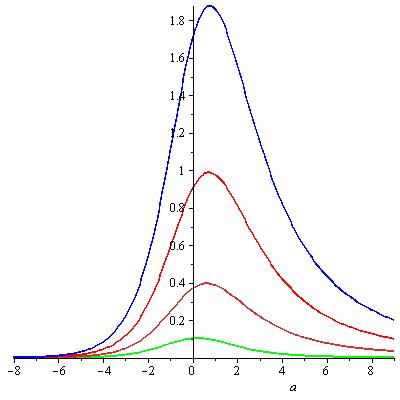
\includegraphics[scale=0.5]{plots_of_V}
				\caption{These are the selfmade plots of $V(r_*)$ for $l=\{0,1,2,3$\}.} \label{plots_of_V}
			\end{center}
	\end{figure} %eigener Plot eingefügen	
	So from now on we remain within the case of $m^2=0$, the massless case.
	Here the asymptotic behavior of the potential is
		\begin{equation} \label{potential_near_infinity}
			V\approx
			\begin{cases}
				\frac{l(l+1)}{r^2_*} &r_* \rightarrow \infty \\
				(l^2 + l + 1) e^{r_*-1} &r_* \rightarrow - \infty
			\end{cases}
		\end{equation}
	If you wonder, why $r_*$ can go to infinity, then send $r$ in the tortoise coordinate \eqref{r_*tortoise} to 1 (which would be the Schwarzschild radius). You will get minus infinity. So this just means, that $r$ approaches $r_s$. 
	
	So the first approachment in \eqref{potential_near_infinity} leads to the vanishment of the potential at spatial infinity polynomially in $r_*$, but near the horizon it vanishes exponentially.
	The barrier between these two regions of \eqref{potential_near_infinity} can be seen in \textbf{Figure \ref{plots_of_V}}. For $\ell \gg 1$ we will find the peak at $r = \frac{3}{2}$ (which means in the figure at approx. $r_*= 0.8$) with a height of order $\ell^2$.
	
	For modes with less energy then the height of the barrier, we have two regions outside the black hole to look at: 
	\begin{enumerate}[1.)]
		\item $r \gg \frac{3}{2}$ : Here the geometry is weakly curved, so modes propagate like in Minkowski space.
		\item $1 < r < \frac{3}{2}$ : This near-horizon region can be called "thermal atmosphere" or "the zone". The first name was given because the modes, which propagate mostly near the horizon, must deal with a Boltzmann distribution with temperature $T_{\text{Hawking}} \approx 1$.  
	\end{enumerate} 	
	If we one approches this problem on the base of Schrödinger equation \eqref{schroedinger_eq}, it can be viewed as a scattering problem, see \textbf{Figure \ref{scattering}}. The modes can come from two directions and leave in two directions namely: coming from a white hole horizon at $r_*\rightarrow -\infty$ or from $J_-$ at $r_*\rightarrow \infty$, which is the past null infinity if you remember, and leaving into the black hole horizon at $r_* \rightarrow -\infty$ or through $J_+$ at $r_* \rightarrow \infty$, which would be the future null infinity.
	
	If we want to know how one unique mode behaves, we need to look set boundary conditions. There are two possible directions, the particles can come from:
	\begin{enumerate}[(i)]
		\item They are send in from the right ({\color{blue} blue} arrow). The possibility if the black hole absorbs them ({\color{red} red} arrow), is given by the transmission coefficient which we get from the Schrödinger problem. But most of them will not ({\color{orange} orange} arrow), so the biggest part of the modes will live at $r \gg 1$.
		\item This time, we don't allow particles come from the right. Instead they are coming out of the white hole, from the left ({\color{forestgreen} green} arrow). Most of it will be reflected off the barrier and fall back into the black hole ({\color{red} red} arrow). Some will tunnel through and go to infinity ({\color{orange} orange} arrow). There the biggest part of these modes is near the horizon which is why they are often called "zone modes" or "modes in the zone".
	\end{enumerate} 
	
	In the following chapter we will find out, which modes are more important.  
	\begin{figure} [tbp]
		\begin{center}
			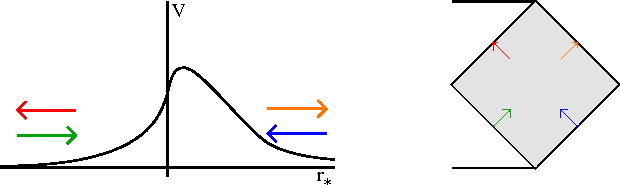
\includegraphics[scale=1.6]{schscat}
			\caption{On the right side there is shown a part of the Schwarzschild Penrose diagram. The grey region is $-\infty < r_* <\infty$. At the left you can see one potential V build on $r_*$ and the possible directions the modes can go are the colorful arrows. The {\color{forestgreen} green} one is coming from the white hole, the {\color{blue} blue} one comes from the null past infinity while the {\color{red} red} one goes into the black hole and the {\color{orange} orange} one goes to the null future infinity.} \label{scattering}
		\end{center}
	\end{figure}

%\section{Information problem}
\section{Information problem}

	\subsection{Black hole radiation} 
	%hawkings paper [1]
	\begin{figure}
		\begin{center}
			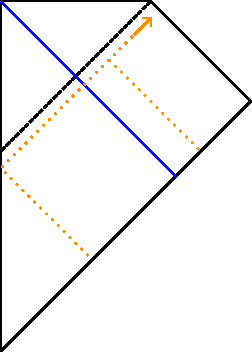
\includegraphics[scale=1]{collapse2}
			\caption{Bla} \label{plots_of_V}
		\end{center}
	\end{figure}

	\subsection{Entropy and thermodynamics \checkmark}
	If a black hole has a temperature and an energy, it must also have an entropy. So let's remember the inner energy in statistical mechanics\footnote{$\diff E = 
	T \diff S - p \diff V + \mu \diff N$} and derive it to:
		\begin{equation}
			\frac{\diff S}{\diff E} = \left. \frac{1}{T} \right|_{V,N=const.}
		\end{equation}
	For the black hole we have $T = \frac{1}{8 \pi G M}$ and $M=E$. If we assume that $S(E=0) = 0$, we can write:
		\begin{align}
			\frac{\diff S}{\diff M} &= 8 \pi G M \nonumber \\
			&\Leftrightarrow \int_0^S \diff S' = \int_0^M 8 \pi M' dM' \nonumber\\
			&\Leftrightarrow S = 4 \pi G M^2 & & \Bigm| r_s = 2GM \nonumber\\
			&\Leftrightarrow S = \frac{r_s^2 \pi}{G}  & & \Bigm| A=4 \pi r_s^2 \text{~and~} l_p = \sqrt{8 \pi G} \nonumber\\
			\Leftrightarrow~
			S &= \frac{A}{4G} = 2 \pi \frac{A}{l_p} \label{entropy}
		\end{align}
	For a black hole of the mass of our sun, this entropy would be $10^{78}$ which is enormous! If we take the sun like it is, the entropy would ``just'' be $10^{60}$. 
	
	Historical the entropy of a black hole was discovered before its temperature. With help of classical general relativity, we can see that the area of an event horizon of a black hole never decreases which looks quite like the second law of thermodynamics. Together with certain formal definition of the entropy, where it is proportional to the horizon area and a temperature indirect proportional to the Schwarzschild radius, the first law of thermodynamics with $\diff M = T \diff S$ is satisfied, too. 
	
	Jacob Bekenstein was holding out that this entropy should be that kind of statistical entropy of a black hole, that counts the number of ways it could have formed itself. 
	In a thought experiement he was throwing some systems with own entropy into a black hole and discovered that the interior entropy was growing faster, than the exterior entropy was sinking because of the systems loss. 
	So this means, that the entropy must be given by some constant proportional to the horizon area in Planck units.
	Bekenstein called this the \textit{Genereralized Second Law}.
	
	As Hawking published his paper about the temperature of a black hole, Bekensteins theory strongly reinforced. This is why the entropy of a black hole is often called \textbf{Bekenstein-Hawking entropy}. 
	
	In \textit{string theory} this idea of an entropy counting microstates is strong supported. For example in many situations where we count the states of a long vibrating string we can see how big the entropy of a black hole is. In some supersymmetric cases it is even possible to compute the $\frac{1}{4}$ in equation \eqref{entropy}.
	
	\subsection{Evaporation}
	%hawkings paper [2]

	%\clearpage
	\subsection{What happens to the information while evaporation? N}
	Steven Hawking said in his paper\marginpar{[2]}, it is inconsistent with quantum mechanics, that the black hole's entropy counts the number of ways it could have been formed which most people would think in the first place. 
	
	The idea behind these thoughts is that the outgoing radiation of a black hole is completely independent of details of the initial state of photons. 
	In explicit we make a diagonal density matrix
		\begin{equation} \label{density matrix informprobl}
			\rho \propto \bigotimes_{\omega, l, m} \left(
			\sum_n \ket{n} \bra{n}_{\omega, l, m} P_{abs} (\omega, l) e^{-\beta \omega n}
			\right)
		\end{equation}
	which leads to the emission rate\marginpar{das gehört weiter nach oben} 
		\begin{equation}
			\frac{\diff E}{\diff t} = 
			\frac{\omega \diff \omega}{2\pi} 
			\frac{P_{abs}(\omega, l)}{e^{\beta \omega}-1}
		\end{equation}
	where $\beta = \frac{1}{T_{Hawking}}$, and $P_{abs}(\omega, l)$ is the absorption
	probability of a ``blue'' mode.
		
	This should remind you of the Rindler result which means that this reduced density matrix for the right or left Rindler wedge is just a thermal density matrix. But back then, we did not calculate in the gravity, so there will be catastrophic consequences once we turn on the gravity again.
		
	Now, if a black hole was originally formed in some pure state $\ket{\psi}$, its outside radiation field becomes more and more mixed as we move forward in time. Because we are normally only looking at the late radiation outside of the black hole, this doesn't seem problematic. 
		
	While the black hole evaporates and becomes smaller, its entanglement entropy is always increasing as seen in \eqref{density matrix informprobl}. The problem is, its size decreases until it is Planckian\footnote{The planck scale beginns at the planck length $l_p = \sqrt{\frac{\hbar G}{c^3}} \approx 1,6 \cdot 10^{-35}m$, while a proton is about the size of $8,4 \cdot 10^{-16}m$} and in those kinds of systems our common physics can't help us any more.
	
	What happens to the entropy now? One of two things must happen:
		\begin{enumerate}[(1)]
			\item The evaporation stops at Planck size. This rest is also called ``remnant'' and its entanglement entropy must be enormously big, bigger than that of a black hole with a comparable mass. \label{evap. planck size}
			\item The black hole finishes the evaporation till there is nothing left. The law of energy conservation prohibits that the last boost of photons contains enough entanglement entropy for reproducing the initial state. But if information can not get lost, we would have to violate the quantum mechanics here.
			So in the end we would have a mixed state with an entropy comparable to the one of the initial horizons entropy. \label{evap. finished}
		\end{enumerate}
	The option number \eqref{evap. planck size} is in fact possible, but it would mean that there are objects with an infinit amount of states below any finite energy.
	Also if a black hole can form out of photons and gravitons why should it not be possible for it to disapear entirely back into photons and gravitons.
	
	Option \eqref{evap. finished} in contrast seems to be the better choice, but it also means that black holes can destroy information. So one must admitt that gravity and quantum mechanics are inconstistent, they have no theory in common.
	
	Let's have a look at an other option, which is nearly similar to option number \eqref{evap. finished}:
		\begin{enumerate}[(3)]
			\item While evaporating, the information is hidden in some entanglement between the Hawking photons blasted by the black hole (or the rest of it).
			In the end we have a pure state of the radiation field instead of a mixed state like in \eqref{evap. finished}. This is just possible if we don't look at too many photons at once, because in complicated states any small subsystem looks thermal, so it can justify \eqref{density matrix informprobl}. 		
		\end{enumerate}				
		

\newpage
\thispagestyle{empty}
\printbibliography
\end{document}

%%% Local Variables: ***
%%% TeX-master: "main.tex" ***
%%% End: ***

